%(BEGIN_QUESTION)
% Copyright 2006, Tony R. Kuphaldt, released under the Creative Commons Attribution License (v 1.0)
% This means you may do almost anything with this work of mine, so long as you give me proper credit

{\it Integralfunksjonen} dukker opp i en rekke fysiske systemer vi møter i prosessmåling og regulering. En slik anvendelse er væskestrøm. Her vises en beholder for væske, utstyrt med en vortex-flowmåler for å måle innkommende væskestrøm og en nivåmåler for å måle væskevolumet som akkumuleres i beholderen:

$$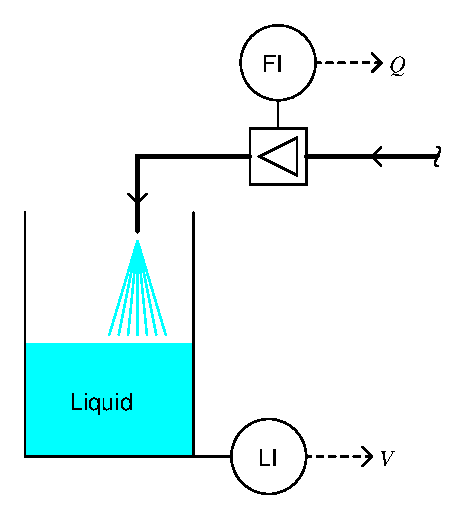
\includegraphics[width=15.5cm]{i01578x01.eps}$$

Hvis du tegner både væskestrømmen ($Q$) og væskevolumet ($V$) som akkumuleres i beholderen over tid, hvilken av disse to variablene vil være integralet av den andre med hensyn på tid? Hvordan skriver du dette matematisk, som et kalkulusuttrykk?

\underbar{file i01578}
%(END_QUESTION)





%(BEGIN_ANSWER)

Volum er tidsintegralet av strømningsrate i dette systemet:

$$V = \int Q \> dt$$

%(END_ANSWER)





%(BEGIN_NOTES)

Det bør nevnes for studentene at det finnes virkelige enheter kalt {\it integratorer}, som tar et signal fra en flowmåler og omgjør det til en måling av totalt volum.

%INDEX% Mathematics, calculus: integral (accumulated volume as the integral of flow)

%(END_NOTES)
